% !TeX encoding = UTF-8

%% ------------------------------------------------------------------------
%% Copyright (C) 2021,2022 SJTUG
%% 
%% SJTUBeamer Example Document by SJTUG
%% 
%% SJTUBeamer Example Document is licensed under a
%% Creative Commons Attribution-NonCommercial-ShareAlike 4.0 International License.
%% 
%% You should have received a copy of the license along with this
%% work. If not, see <http://creativecommons.org/licenses/by-nc-sa/4.0/>.
%%
%% For a quick start, check out src/doc/sjtubeamerquickstart.tex
%% Join discussions: https://github.com/sjtug/SJTUBeamer/discussions
%% -----------------------------------------------------------------------

\documentclass[xcolor=dvipsnames,svgnames,aspectratio=169]{ctexbeamer}
% 可以通过 fontset=macnew / fontset=ubuntu / fontset=windows 选项切换字体集

\usepackage{tikz}
\usepackage[normalem]{ulem}
\usetikzlibrary{arrows}
\usepackage{amsmath}
\usepackage{amssymb}
\usepackage{mathtools}
\usepackage{mflogo}
\usepackage{graphicx}
\usepackage{ccicons}
\usepackage{hologo}
% \usepackage{colortbl}
\usepackage{shapepar}
\usepackage{hyperxmp}
\usepackage{booktabs}
\usepackage{qrcode}
\usepackage{listings}
% \usepackage{tipa}
\usepackage{multicol}
\usepackage{multirow}
\usepackage{datetime2}
\usepackage{fontawesome5}
\usepackage{hyperref}
\usepackage{makecell}
\setbeamercovered{transparent=0}

% 参考文献设置,使用 style=gb7714-2015 样式为标准顺序编码制,
% 使用 style=gb7714-2015ay 样式可以改为著者-出版年制。
\usepackage[backend=biber,style=gb7714-2015]{biblatex}
\addbibresource{thesis.bib}

\graphicspath{{figures/}}

\hypersetup{
  pdfsubject = {上海交通大学图书馆专题培训讲座},
  pdfauthor = {Alexara Wu},
  pdfcopyright = {Licensed under CC-BY-SA 4.0. Some rights reserved.},
  pdflicenseurl = {http://creativecommons.org/licenses/by-sa/4.0/},
  unicode = true,
  psdextra = true,
  pdfdisplaydoctitle = true
}

\pdfstringdefDisableCommands{
  \let\\\relax
  \let\quad\relax
  \let\hspace\@gobble
}

\renewcommand{\TeX}{\hologo{TeX}}
\renewcommand{\LaTeX}{\hologo{LaTeX}}
\newcommand{\BibTeX}{\hologo{BibTeX}}
\newcommand{\XeTeX}{\hologo{XeTeX}}
\newcommand{\pdfTeX}{\hologo{pdfTeX}}
\newcommand{\LuaTeX}{\hologo{LuaTeX}}
\newcommand{\MiKTeX}{\hologo{MiKTeX}}
\newcommand{\MacTeX}{Mac\hologo{TeX}}
\newcommand{\beamer}{\textsc{beamer}}
\newcommand{\XeLaTeX}{\hologo{Xe}\kern-.13em\LaTeX{}}
\newcommand{\pdfLaTeX}{pdf\LaTeX{}}
\newcommand{\LuaLaTeX}{Lua\LaTeX{}}

\def\TeXLive{\TeX{} Live}
\let\TL=\TeXLive
\newcommand{\SJTUThesis}{\textsc{SJTUThesis}}
\newcommand{\SJTUThesisVersion}{1.1.0}
\newcommand{\SJTUThesisDate}{2022/3/26}
\newcommand{\SJTUBeamer}{\textsc{SJTUBeamer}}
\newcommand{\SJTUBeamerVersion}{3.0.0}
\newcommand{\SJTUBeamerDate}{2022/11/22}

\newcommand\link[1]{\href{#1}{\faLink}}
\newcommand\pkg[1]{\texttt{#1}}

\def\cmd#1{\texttt{\color{structure}\footnotesize $\backslash$#1}}
\def\env#1{\texttt{\color{structure}\footnotesize #1}}
\def\cmdxmp#1#2#3{\small{\texttt{\color{structure}$\backslash$#1}\{#2\}
\hspace{1em}\\ $\Rightarrow$\hspace{1em} {#3}\par\vskip1em}}

\lstset{
  language=[LaTeX]TeX,
  basicstyle=\ttfamily\footnotesize,
  tabsize=2,
  keywordstyle=\bfseries\ttfamily\color{cprimary},
  commentstyle=\sl\ttfamily\color[RGB]{100,100,100},
  stringstyle=\ttfamily\color[RGB]{50,50,50},
  extendedchars=true,
  breaklines=true,
}

\usetheme[maxplus]{sjtubeamer}
% 使用 maxplus/max/min 切换标题页样式
% 使用 red/blue 切换主色调
% 使用 light/dark 切换亮/暗色模式
% 使用外样式关键词以获得不同的边栏样式
%   miniframes infolines  sidebar
%   default    smoothbars split	 
%   shadow     tree       smoothtree
% 使用 topright/bottomright 切换徽标位置
% 使用逗号分隔列表以同时使用多种选项

% \tikzexternalize[prefix=build/]
% 如果您需要缓存 tikz 图像,请取消注释上一行,并在编译选项中添加 -shell-escape。

\author{答辩人:刘思雨\quad 学号:121033910117}
\institute[SJTU-PLV]{导师:汪宇霆}
\date{\the\year 年 \the\month 月}
\subject{LaTeX, 论文排版, SJTUThesis}

\title[JHC硕士毕业答辩] % 页脚显示标题
{\textbf{基于静态单赋值中间语言的函数式编译器验证方法}} % 首页标题

\subtitle{John Hopcroft Center硕士毕业答辩}

\begin{document}

% 使用节目录
\AtBeginSection[]{
  \begin{frame}
    %% 使用传统节目录,也可以将 subsectionstyle=... 换成 hideallsubsections 以隐藏所有小节信息
    \tableofcontents[currentsection,subsectionstyle=show/show/hide]
    %% 或者使用节页
    % \sectionpage
  \end{frame}
}

% 使用小节目录
\AtBeginSubsection[]{		       % 在每小节开始
  \begin{frame}
    %% 使用传统小节目录
    \tableofcontents[currentsection,subsectionstyle=show/shaded/hide]
    %% 或者使用小节页
    % \subsectionpage
  \end{frame}
}

\maketitle

\begin{frame}{目录}
  \tableofcontents[hideallsubsections]	% 隐藏所有小节信息
\end{frame}

% !TeX encoding = UTF-8
% !TeX root = ../main.tex

\section{研究课题概述}

\begin{frame}{背景:编译器的中间语言}
  \textcolor{DarkBlue}{延续传递风格(Continuation-Passing Style, CPS)}
  \begin{itemize}
    \item CPS是\textcolor{Maroon}{函数式}编译器中常用的中间语言(Intermediate Representation, IR)。
    \item 每一步计算和控制流跳转都要被\textcolor{Maroon}{显式命名}。
    \item CPS中间语言有利于进行\textcolor{Maroon}{控制流分析}。
  \end{itemize}
  \vspace{2ex}
  \textcolor{DarkBlue}{静态单赋值(Static Single Assignment, SSA)}
  \begin{itemize}
    \item SSA是\textcolor{Maroon}{LLVM、GCC}等主流编译器基础设施常用的中间语言。
    \item 每一个变量都只能被\textcolor{Maroon}{赋值一次}。
    \item SSA中间语言有利于进行\textcolor{Maroon}{数据流分析}。
  \end{itemize}
\end{frame}

\begin{frame}{研究动机}
    \begin{itemize}
      \item SSA程序可以用函数式程序表示。CPS和SSA程序在结构上有对应之处。
      \item 目前\textcolor{Maroon}{没有}从CPS到SSA\textcolor{Maroon}{经过形式化验证}的转换。
      \item 我们希望经验证的函数式编译器能够利用SSA的优势。
    \end{itemize} 
    \begin{figure}
      \centering
      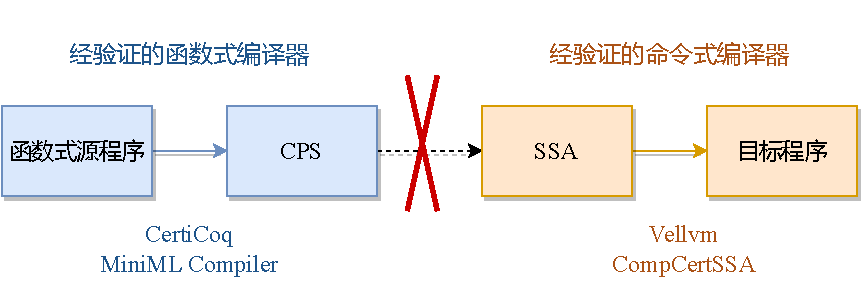
\includegraphics[width=0.8\linewidth]{figures/motiva.pdf}
      \label{fig:moti1}
    \end{figure}
\end{frame}

\begin{frame}{编译器验证技术}
  \textcolor{DarkBlue}{编译器形式化验证}常用技术:
  \begin{itemize}
    \item 基于逻辑关系的验证。与现有的经验证SSA基础设施所用方法不匹配。
    \item 基于\textcolor{Maroon}{模拟(simulation)}的验证。
  \end{itemize}
  \vspace{2ex}
  函数式语言与命令式语言的\textcolor{DarkBlue}{程序状态}组成部分\textcolor{DarkBlue}{差异较大}:
  \begin{itemize}
    \item \textcolor{Maroon}{CPS}:代码项,延续变量信息
    \item \textcolor{Maroon}{SSA}:程序计数器,符号表,调用栈...
  \end{itemize}
  想要使用模拟技术,需要把两种不同的程序状态正确地\textcolor{DarkBlue}{匹配}起来。
\end{frame}

\begin{frame}{主要贡献 1}
  \large
  设计并验证了\textcolor{DarkBlue}{CPS到SSA}语言的转换算法。
  \begin{figure}
    \centering
    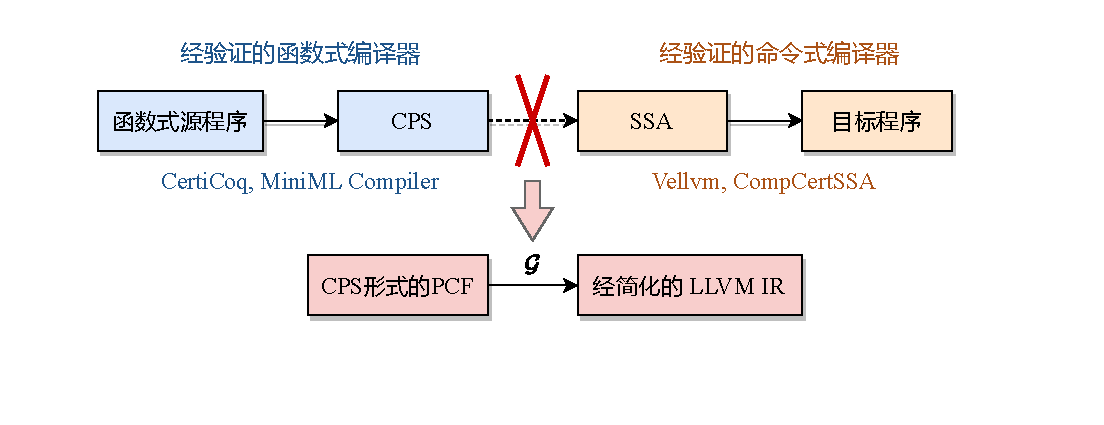
\includegraphics[width=0.95\linewidth]{figures/part.pdf}
  \end{figure}  
\end{frame}

\begin{frame}{主要贡献 2}
  \large
  利用该经验证的编译过程构建了\textcolor{DarkBlue}{PCF到LLVM IR}的函数式编译器。
  \begin{figure}
    \centering
    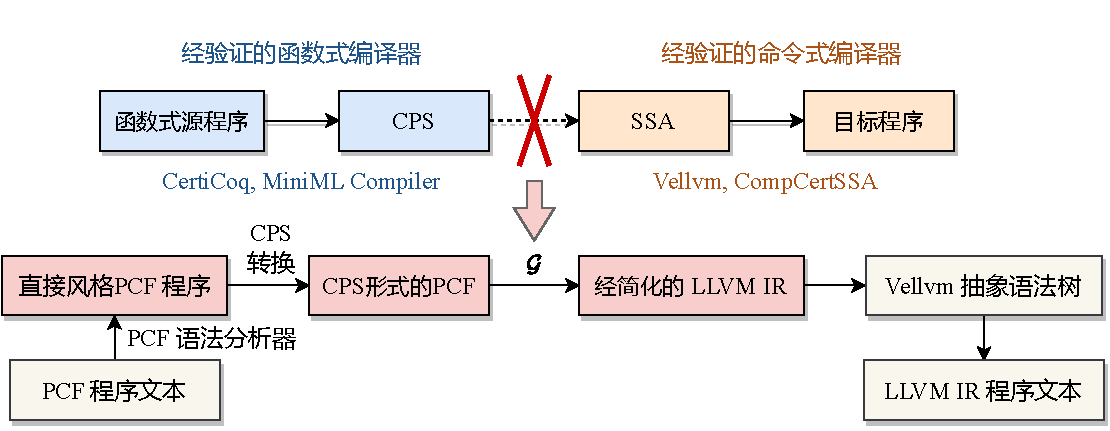
\includegraphics[width=0.95\linewidth]{figures/whole.pdf}
  \end{figure}  
\end{frame}



% !TeX encoding = UTF-8
% !TeX root = ../main.tex

\section{CPS到SSA的转换算法}
% !TeX encoding = UTF-8
% !TeX root = ../main.tex

\section{CPS到SSA转换过程的验证}
% !TeX encoding = UTF-8
% !TeX root = ../main.tex

\section{完整编译链及其实现}

\begin{frame}
    \frametitle{基于SSA的函数式编译器}
    \begin{figure}
        \centering
        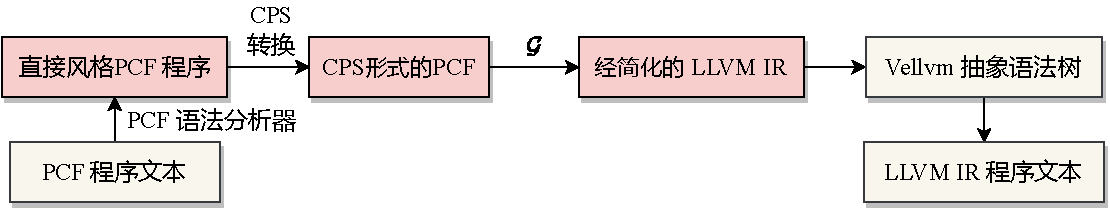
\includegraphics[width=0.9\linewidth]{figures/summary.drawio.pdf}
    \end{figure}
    \begin{itemize}
        \item 构建了一个\textcolor{Maroon}{从PCF函数式程序到LLVM IR的编译器},并对其\textcolor{Maroon}{核心编译步骤进行形式化验证}。
        \item PCF语法分析器(Parser)将PCF程序文本提取为抽象语法树。
        \item 对直接风格PCF程序进行CPS转换和CPS到SSA的转换,并进行验证。
        \item 将SSA连接到Vellvm抽象语法树,得到LLVM IR。
    \end{itemize}
\end{frame}

\begin{frame}
    \frametitle{编译器实现及代码统计}
    \begin{itemize}
        \item 主要使用交互式定理证明器\textcolor{Maroon}{Coq}实现,代码行数统计见下表(不包括所使用的CompCert中的定义和定理)。
        \item PCF语法分析器(Parser)在\textcolor{Maroon}{OCaml}中实现。
        \item 与LLVM IR的连接使用了Coq中的\textcolor{Maroon}{Vellvm}抽象语法树及其相关工具。
    \end{itemize}
    \vspace{1ex}
    
    \begin{table}
        \linespread{1.25}
        \scriptsize
        \centering
        % \vspace{-20pt}
        \begin{center}
        \begin{tabular}{|l|l|l|l|}
        \hline
        类别 & 内容 & LOC & 占比(\%) \\
        \hline
        语言定义 & PCF, CPS, SSA & 702 & 23.9 \\
        \hline
        转换算法 & \makecell[l]{PCF$\rightarrow$CPS, CPS$\rightarrow$SSA,\\SSA$\rightarrow$Vellvm LLVM IR}  & 717 & 24.5 \\
        \hline
        定理证明 & \makecell[l]{PCF$\rightarrow$CPS及CPS$\rightarrow$SSA前向模拟,\\ 前向模拟的合并及后向模拟} & 1513 & 51.6 \\
        \hline
        \end{tabular}
        \end{center}
\end{table}
\end{frame}
% \include{contents/thesis}
% !TEX root = ../main.tex

\chapter{全文总结} \label{ch:summary}

\section{主要结论}

\section{研究展望}


% \begin{frame}
%   \frametitle{参考文献}
%   \printbibliography[heading=none]
% \end{frame}

\makebottom

\end{document}
